\section{Introduction}
\subsection{Tree-depth definition}
For undirected graph $G$, the tree-depth $td(G)$ is a graph invariant. Intuitively, we may think of it as the parameter that says how similar $G$ is to a star. The lower tree-depth is, the more "starlike" $G$ is.
Tree-depth value can range from 1 to $|G|$.
To explain the most common tree-depth definition, it is necessary to introduce term tree-depth decomposition. Tree-depth decomposition of graph $G$ is a forest $F$ with the following property:\\\\
\emph{If there is an edge $uv$ in $G$ then vertices $u$ and $v$ have ancestor-descendant relationship between each other in $F$.}\\\\
Using this definition, the tree-depth of $G$ is a depth of the forest with minimal depth among all tree-depth decompositions of $G$.\\\\
Tree-depth can also be defined in a recursive manner. It is worth mentioning, because we make strong use of it in our dynamic algorithm, presented later in this documentation. The definition looks as follows:\\\\
\begin{equation}
td(G) =
\begin{cases}
1 & \text{if $|$G$|$=1}\\
1+\min_{v \in V} td(G-v) & \text{if G is connected}\\
\max_{i} td(G_{i})  & \text{otherwise}
\end{cases}\label{td_def}
\end{equation}
\\
\subsection{Examples}
In this paragraph we will provide some obvious facts and examples of tree-depth decompositions in order to give reader a better intuition.\\\\
The only connected graph which tree-depth equal to 1 is complete graph \emph{K$_{1}$}\\
Stars are the only connected graphs with tree-depth equal to 2.  For these graphs, graph and its best tree-depth decomposition are isomorphic.\\\\
Antoher thing is that for every graph $G$, a trivialy valid tree-depth depcomposition of $G$ is a path $P_{\left|G\right|}$ rooted in its beginning. It is true, because for such a tree every pair of vertices have ancestor-descendant relationship to each other.\\\\
The last fact, to point out is that if $G$ is connected then its tree-depth decomposition $F$ is also connected. It is true, because if $F$ had two components, then there would be two groups of vertices in $G$ without edges between each other, which is contradictiory to $G$ being connected.
\begin{figure}[hbt!]
	\centering
	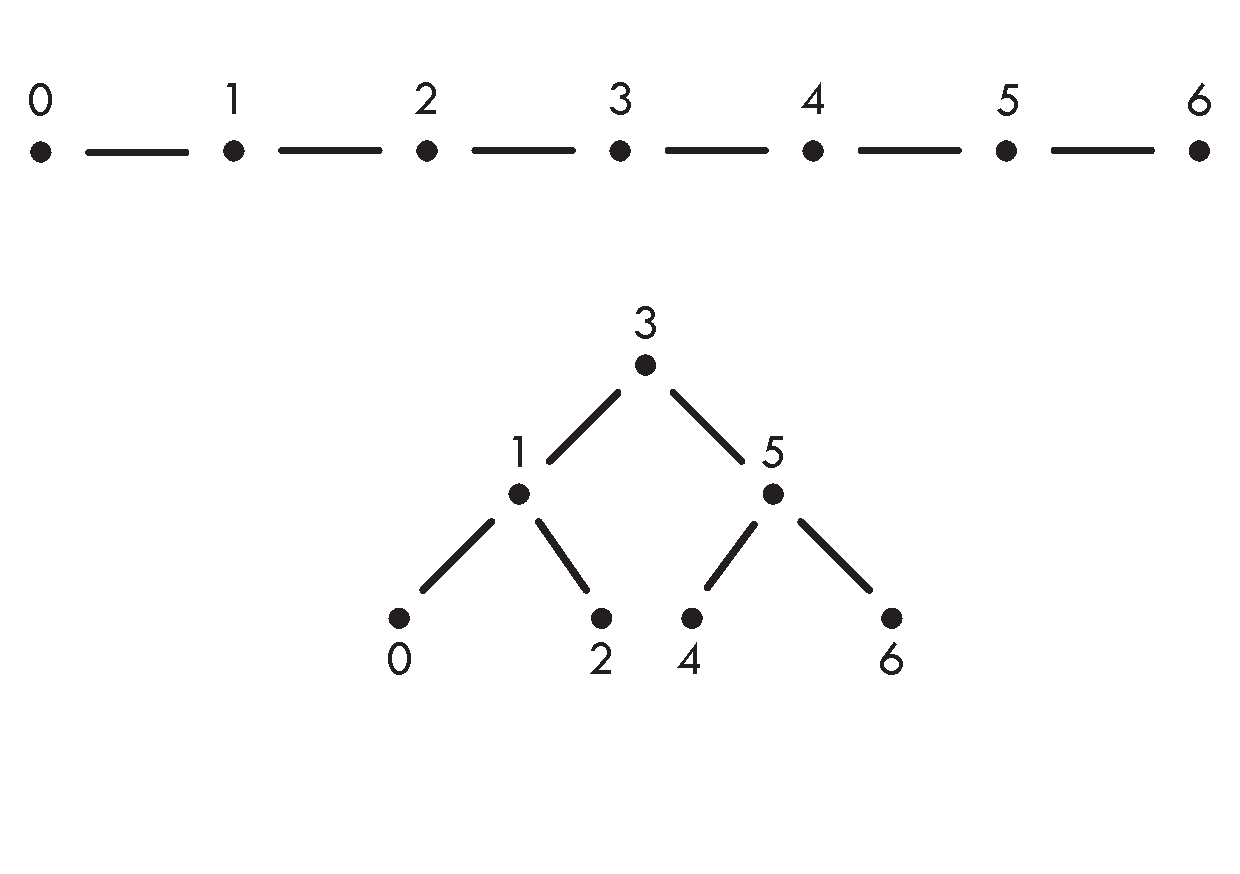
\includegraphics[scale=0.5,valign=t]{sciezka.pdf}
	\caption{P$_{7}$ and its tree-depth decomposition}
\end{figure}
\\\\\\\\
\begin{figure}[hbt!]
	\centering
	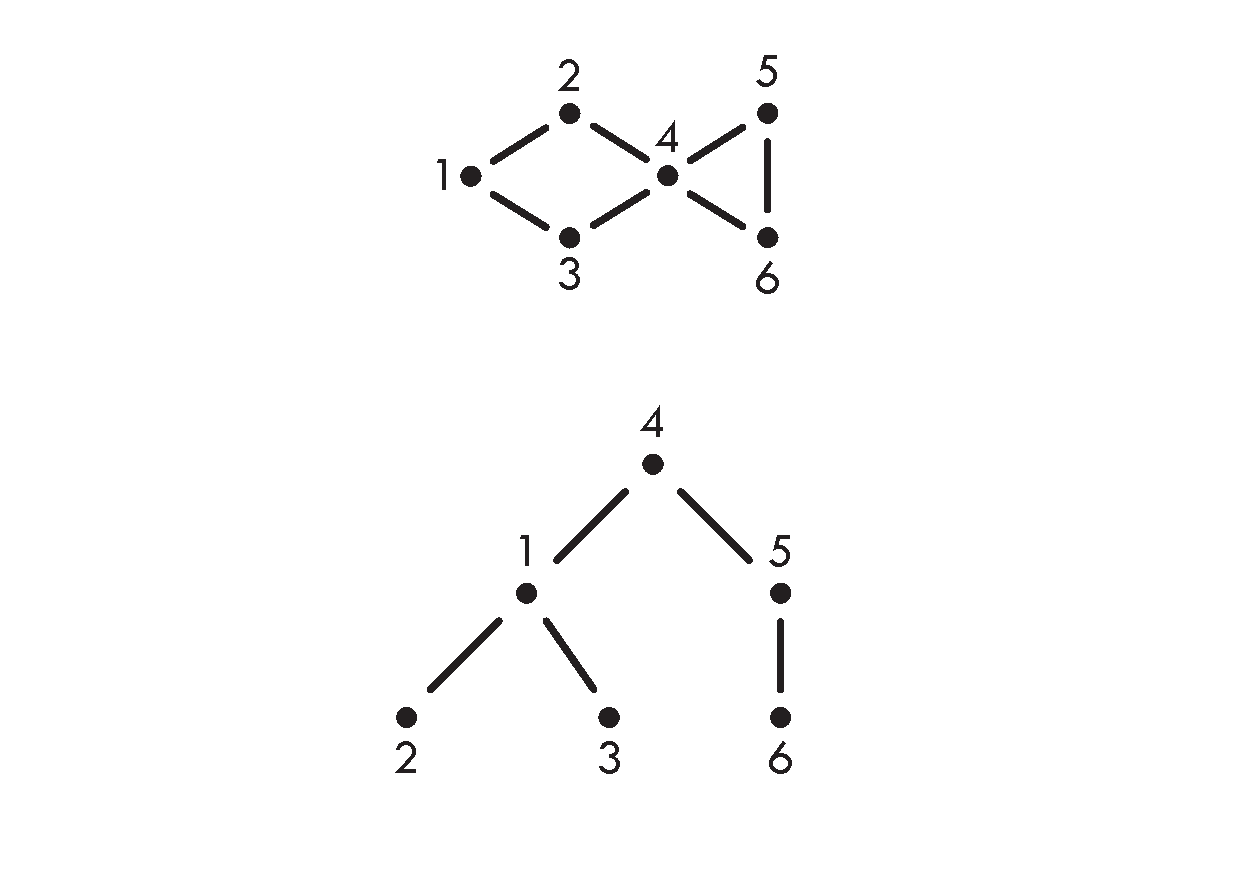
\includegraphics[scale=0.5,valign=t]{rybka.pdf}
	\caption{Fish and its tree-depth decomposition}
\end{figure}

